\section{What Kind of Help do Novices Need?}
\begin{figure}[b!]
\centering
  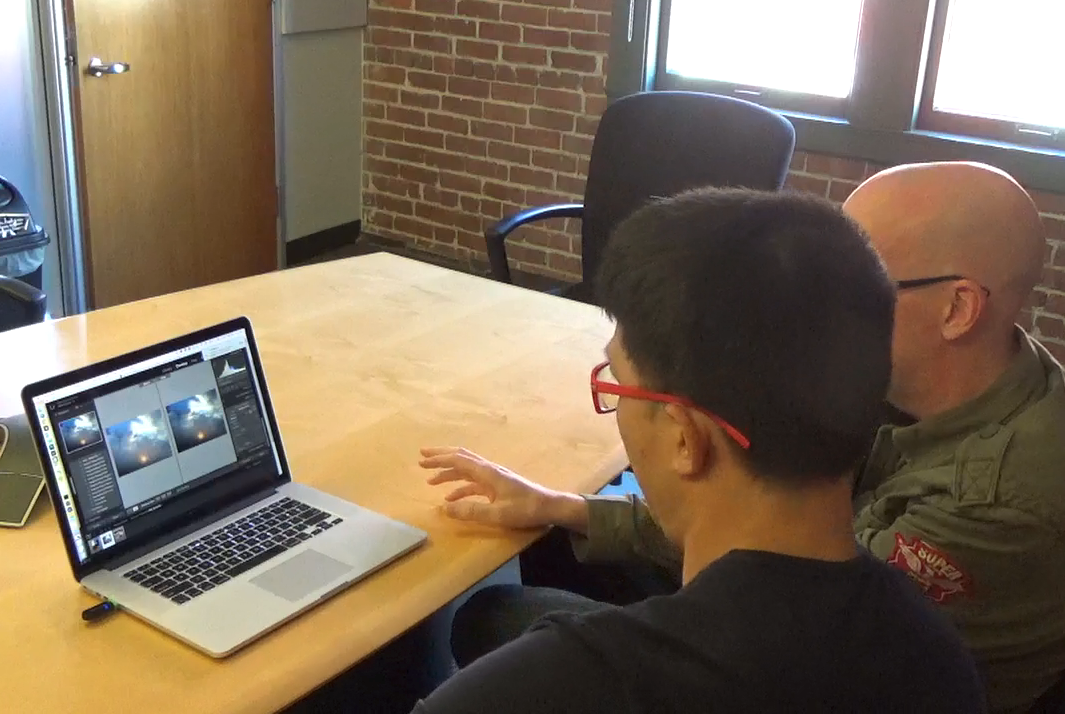
\includegraphics[width=0.6\textwidth]{discoveryspace/figures/obs.png}
  \caption{A novice-expert session. The expert (right) compares the edited photo with the original to illustrate what the edits did.}~\label{fig:discoveryspace_obs}
\end{figure}

To unearth novice-expert differences in creative software usage strategies, we conducted nine 30-minute sessions in which three expert photo editors helped seven novices edit their photos using Adobe Photoshop and Lightroom. Each session included one novice and one expert (\autoref{fig:discoveryspace_obs}). The novice described their goals while the expert controlled the program and communicated with the novice to help achieve them. One-on-one tutoring like these pair discussions is highly effective for teaching \cite{Bloom1984}, and consequently a valuable model for what software could achieve. We observed these interactions to see what novices asked, how experts translated these requests into image editing operations, and whether there were novice-expert language differences or communication challenges. Our intuition is that good software should enable novices to solve challenges like these for themselves. After all the sessions, we reviewed our notes and looked for recurring behaviour patterns. The following four insights were most prominent:
\begin{enumerate}
    \item Novices often did not know what they wanted to do with a photo, and could not picture how it might be improved. In these cases, the experts would provide their own suggestions to get things started.
    \item Novices had very high-level goals (\textit{e.g.}, ``I want to make this person stand out more''), and often did not know what tools or techniques were needed to accomplish them. Experts were able to translate these goals into concrete operations.
    \item A common way to show a novice what an effect will do was to execute it on the photo and compare the result with the original photo, sometimes exaggerating the effect to illustrate the difference before dialing it back down. Novices were sometimes hesitant about an expert's suggestion, but after seeing its effect on the image would become more excited about it.
    \item Novices appreciated both suggestions that were relevant to their goals, \textit{and} suggestions for different effects they would not have otherwise thought of.
\end{enumerate}
